\section{Métodos lineares}

\begin{figure}[H]
\Caption{\label{fig:lineares-tempo}Métodos lineares - Tamanho × Tempo.}
\centering
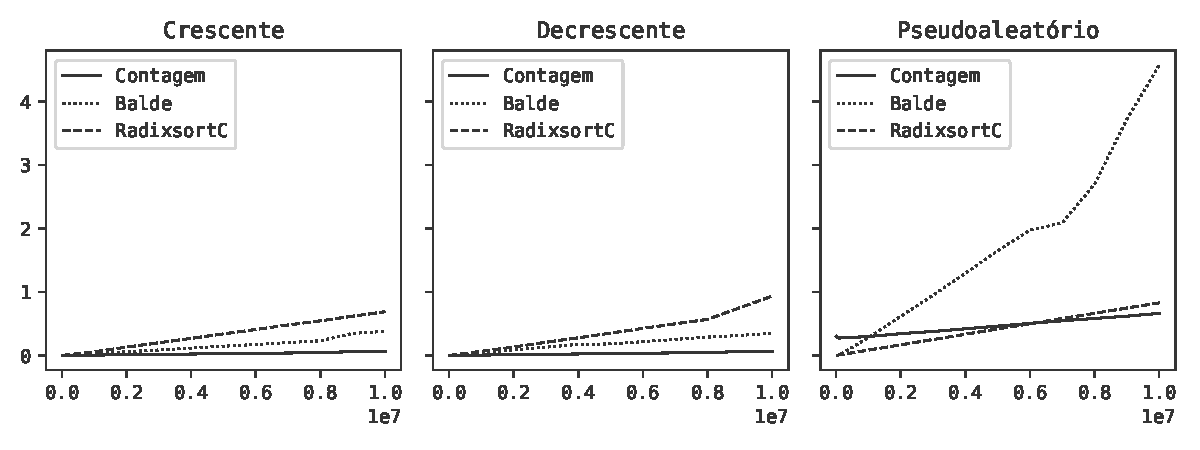
\includegraphics[scale=0.787]{figuras/pdf/lineares.tempo.pdf}
\Fonte{Elaborado pelo autor}
\end{figure}

\begin{figure}[H]
\Caption{\label{fig:lineares-movimentacoes}Métodos lineares - Tamanho × Movimentações.}
\centering
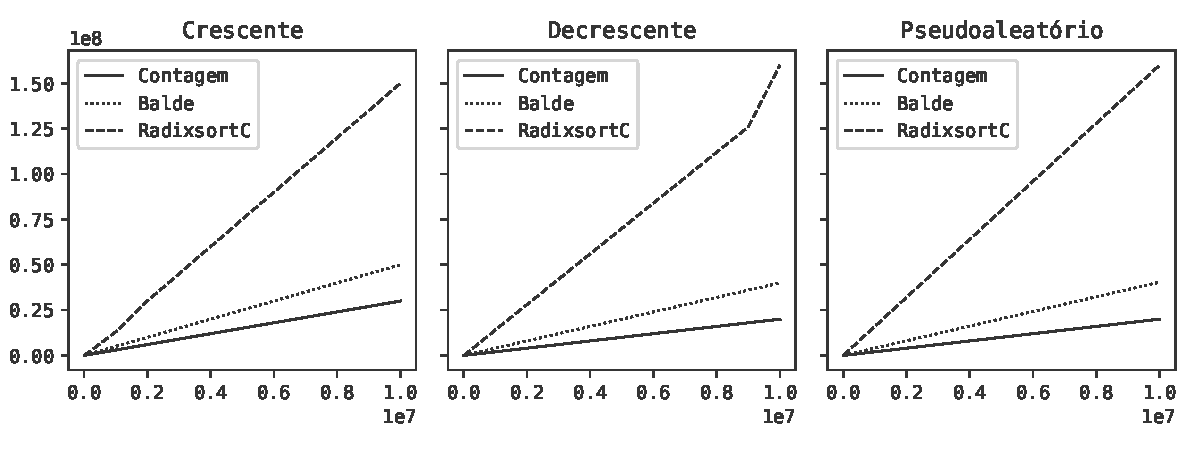
\includegraphics[scale=0.787]{figuras/pdf/lineares.movimentacoes.pdf}
\Fonte{Elaborado pelo autor}
\end{figure}